\chapter{Background / Related Work}
\label{ch:relatedwork}

\section{Two-Dimensional Image Representation on Computers}
\label{sec:2dimages}

At it's most basic form, a sketch can be described as an image usually drawn on a planar two-dimensional surface.
With computer displays, there are two standard methods for generating two dimensional images: raster graphics and vector graphics.
The underlying data structures  have a large impact on the types of tools that can be designed to create, modify, and display the resulting images.

\subsection{Raster Graphics}

Raster graphics is an image format that uses a two-dimensional grid to represent each pixel in the image. 
A raster image is characterized by its width and height in pixels and by its color depth, the number of bytes per pixel. 
The depth value specifies the color for each pixel, usually by identifying the magnitude of the pixel's RGB components. 
The reasoning behind representing images by this method is that today most computer monitors have bitmapped displays. 
Today, although there are many standard formats, almost all displays consist of rectangular arrays of square pixels, and the bandwidth from the display's memory is sufficient enough to dynamically render multi-megapixel images. 
\begin{figure}
\label{fig:raster}
\fbox{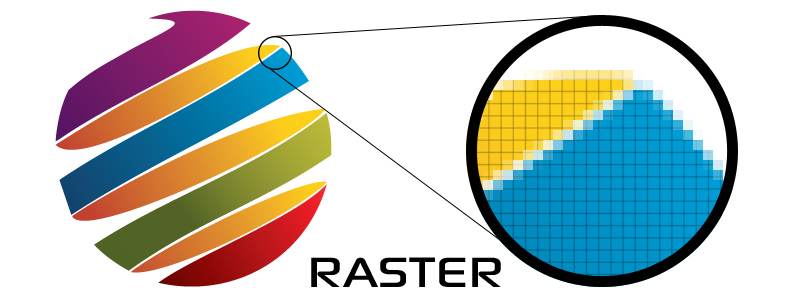
\includegraphics[width=\textwidth]{raster.jpg}}
\caption[Zooming in on a Raster Graphics Image]{When we zoom in on a raster graphics image, we can see the image degradation that occurs from the pixel based storage format. \autocite{printingcollection}}
\end{figure}



When creating and editing raster graphics images, the software directly manipulates pixel values, also known as pixel editing.
This simplifies creating tools for editing raster graphics, since each tool can manually define how pixels are effected based on where and how an input occurs. 
Unfortunately, the ultimate quality of an image based on raster graphics is limited by the fact that the picture is resolution dependent.
The resolution of the image is independent of the resolution of the display, and it is possible for raster images for contain very large amounts of information, as can be seen from the Gigapixel Project \autocite{gigapixel}.
However, even this still has it's limits.
If you were to continuously zoom in on a raster image, eventually the image would eventually suffer from image degradation. 
This resolution dependency also means that raster images are not flexible for working with extremely detailed environments.
It is possible for multiple small details to be contained inside of a single pixel.
Since a pixel can only store one color, all of these small details are lost.


\begin{figure}
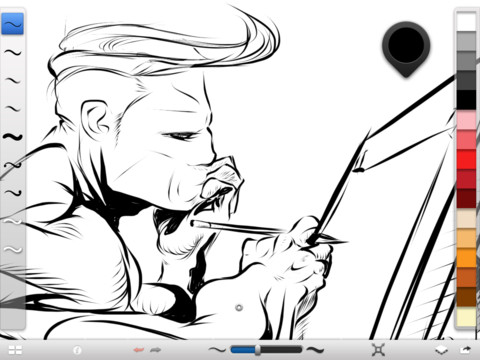
\includegraphics[width=\textwidth]{sketchbook.jpg}
\caption[Creating a Raster Image in Sketchbook]{An artist creates a raster image using Sketchbook. The software comes with a variety of pen styles and tools to help simulate a physical art studio. \autocite{sketchbook}}
\end{figure}



Examples of popular raster graphics software are Corel Painter \autocite{coreal}, Adobe Photoshop \autocite{photoshop}, Microsoft's MSPaint \autocite{mspaint}, the open-source GIMP software \autocite{gimp}, and Autodesk's Sketchbook \autocite{sketchbook}.

\subsection{Vector Graphics}
\begin{figure}
\fbox{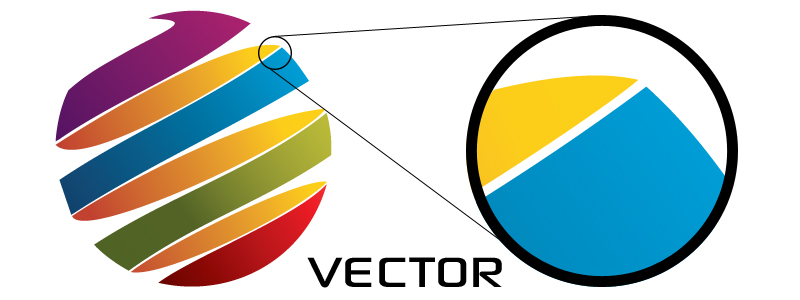
\includegraphics[width=\textwidth]{vector.jpg}}
\caption[Zooming in on a Vector Graphics Image]
{When we zoom in on a vector graphics image, we can see the lines remain smooth, unlike in a similar raster graphics image. (Figure~\ref{fig:raster}) This is because of the underlying mathematical representation of the shapes in the image. \autocite{printingcollection}}
\end{figure}

Vector graphics software uses geometrical primitives such as points, lines, curves, shapes and polygons to represent an image.
Each of these primitives has a defined geometric coordinate within the work space and determines the direction of the displayed vector. 
Vectors can also be assigned a variety of properties such as its color and thickness.
Although the resolution is limited by the computer's numerical precision, it is independent of the actual display. 

Because of the mathematical nature of vector graphics, they are theoretically similar to three-dimensional computer graphics, but the term specifically refers to two-dimensional images; in part to distinguish them from raster graphics.
Vector graphics are primarily used for line art, images drawn with distinct straight or curved lines.
For example, early CAD systems mostly used calligraphic black and white displays and rendered images in vector graphics formats. 
However, today, data in vector graphics form is now converted to raster graphics formats when used outside of vector specific editing software.  

Vector graphics data structures offer a number of advantages compared to raster approaches. 
First, they are based on mathematical expressions, which means they are resolution independent.
Zooming in on the image does not cause image degradation as in raster graphics; the image will remain smooth. 
Second, objects made using vector graphics are independent from their visual representation.
This allows for easy and accurate editing of primitives, provided they are contained in a vector graphics workspace.
For example, assume we have an image of a circle covering a part of a square. In vector graphics, the circle can be moved without effecting the square beneath, because the data structure contains the information about both objects independently from their visual representation.
This type of editing is not possible in a single raster graphics image, because the underlying pixel representation does not contain the definition of objects in the image.

Examples of popular vector graphics editing software are Adobe Illustrator \autocite{illustrator}, Corel Draw \autocite{coreldraw}, and Inkscape \autocite{inkscape}.

\subsection{Adaptively Sampled Distance Fields}

In addition to the most commonly used data structures (raster and vector graphics), methods combining the capabilities of both approaches are beginning to emerge.
An example of this is a new data structure called adaptively sampled distance fields \autocite{asdf} (ADFs).
A distance field is a scalar field that specifies the minimum distance to a shape, where the distance may be signed to distinguish between the inside and outside of the shape.
In ADFs, distance fields are sampled according to local detail and stored in a spatial hierarchy.
ADFs are capable of representing a large class of forms, while reducing the storage size to a fraction of a traditional spatial data structure.

Mischief \autocite{mischief}, a pseudo-vector graphics based drawing application. 
Although its underlying shape representations are mathematical, similar to those in other vector graphics applications, it does not allow for the precise editing of curves and shapes as seen in traditional vector graphics programs such as Adobe Illustrator. 
Instead it attempts to use vector graphics to simulate real world art techniques, similar to Sketchbook.
This is made possible by using ADFs to store the complicated details and shapes of real world brushes.
Mischief is also able to utilize the efficient storage capabilities of ADFs for the implementation of their "infinite canvas"; their infinitely zoom-able, translatable workspace. 
This unique data structure allows for Mischief to achieve incredible detail and unlimited scale.

\begin{figure}
\centering
\fbox{\includegraphics[width=0.45\textwidth]{infinitecanvas1}}
\fbox{\includegraphics[width=0.45\textwidth]{infinitecanvas2}}
\caption[An example of the infinite canvas in Mischief]
{An example of the infinite canvas in Mischief. The work space can be continuously zoomed in upon without loss in quality.}
\end{figure}

\section{3-D Sketching in CAD}

In order to overcome the limitations of 2D sketching, there have been many previous attempts to utilize 3-D sketching in the design process. 
In this section, we will describe some of the better recent examples others have previously either implemented or published.
A common weakness in each of these methods is that to date none of them implement a way to generate geometry directly from the sketch.

\subsection{CATIA Natural Sketch}

\begin{figure}
\centering     %%% not \center
\subfigure[Details are added to a base model.] {\label{fig:catia2}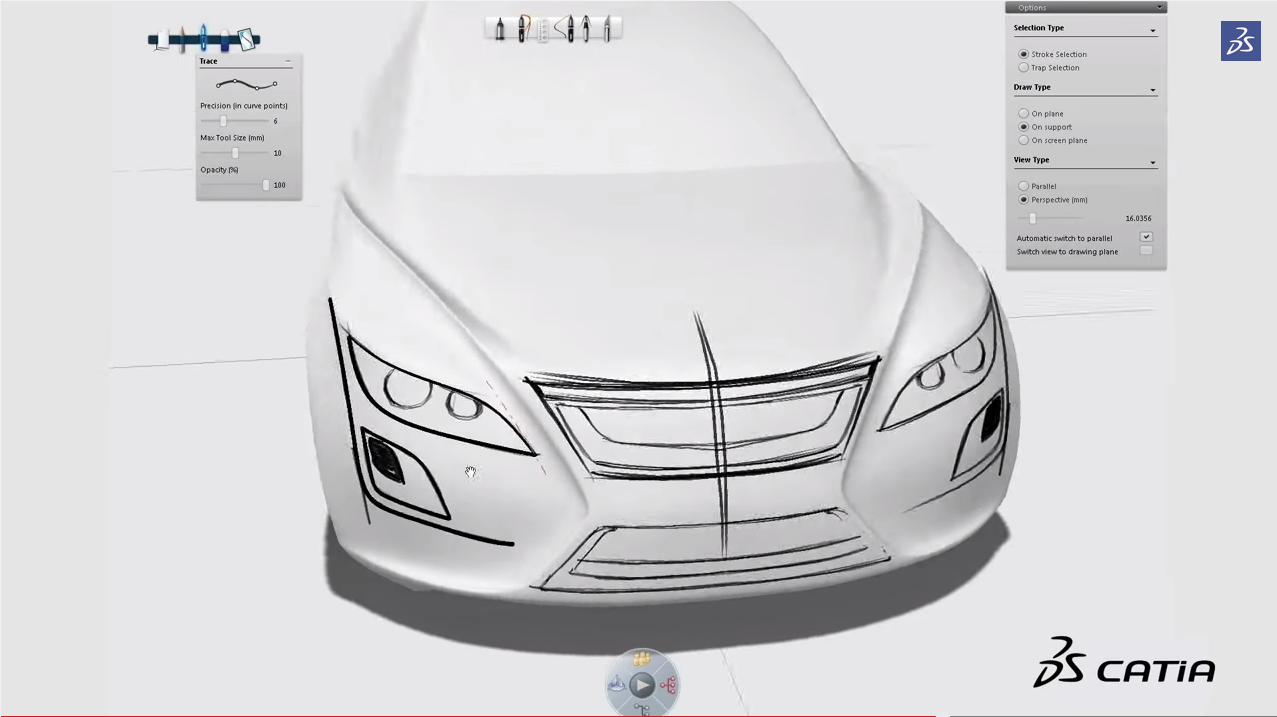
\includegraphics[width=\textwidth]{CATIA2}}
\subfigure[A rough sketch can be traced with editable spline curves.] {\label{fig:catia3}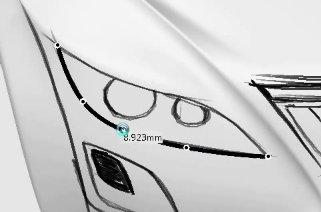
\includegraphics[width=\textwidth]{CATIA3}}
\caption[Using Natural Sketch to Add Detailing to a Car.] {(a) An example of using Natural Sketch to add detailing on the curved surfaces of an existing car model. (b) The rough sketch can then be emulated with Catmull-Clark splines. \autocite{catiareel}}
\end{figure}

Natural Sketch is a feature inside of the CATIA modeling software\autocite{catia}. 
Natural Sketch allows the user to draw on a virtual two-dimensional plane that can be manipulated around the 3-D environment, a surface of an arbitrary 3-D model, and a "clipping plane". 
It's sketching features include the ability to alter the pen style, to automatically change the camera view to align with the drawing plane if one is being used, and to  copy and alter individual strokes.

Natural Sketch uses a two-phase design system. 
First, the user creates a "rough sketch", where lines are rendered exactly as drawn. 
Afterwards, the user can trace over their already drawn lines to produce smooth curves from the initial sketch.
As will be describer in Section~\ref{sec:splines}, CATIA is based on spline technology, which allows for this smooth curve generation.
These curves also contain a user defined number of editable geometric knots, which allow the user to alter the shape of the traced curve.
While this system closely has the capabilities we would like to implement, it is currently only available in a solid modeling environment, making it incompatible with many tools most designers use to create early stage 3-D sketch models.



\subsection{EverybodyLovesSketch}

EverybodyLovesSketch \autocite{lovesketch} is a 3D curve sketching system from the University of Toronto's Dynamic Graphics Project Lab. 
It features a pen based gesture system, allowing the user to execute functions using rapid strokes, circles, and other predefined stroke patterns.
Other features include dynamic sketch plane selection using previously drawn strokes, single view definition of arbitrary extrusion vectors, multiple extruded surface sketching, copy-and-project of 3D curves, free-form surface sketching, and an interactive perspective grid. 
EverybodyLovesSketch is based off of previous work by the same lab, ILoveSketch, which contains the base 3D sketching functionality.

\subsection{Hyve3D}

\begin{figure}
\centering  
\subfigure[A user using an iPad to sketch on a plane inside of the virtual environment.] {\label{fig:hyve1}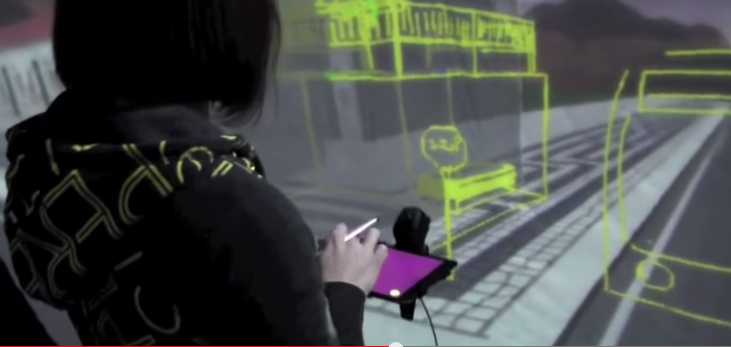
\includegraphics[width=\textwidth]{Hyve3D1}}
\subfigure[Manipulating the drawing plane by manipulating the iPad] {\label{fig:hyve2}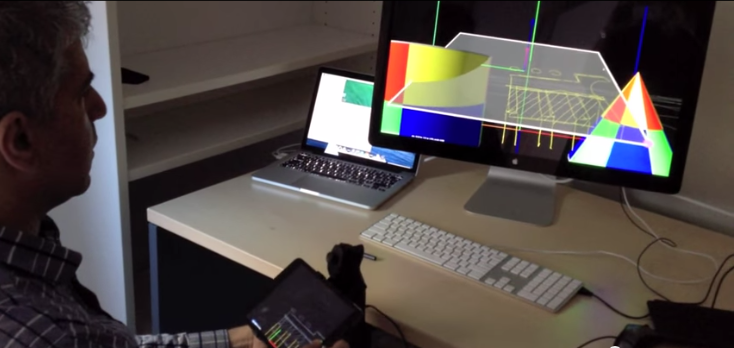
\includegraphics[width=\textwidth]{Hyve3D2}}
\caption[Using Hyve3D to draw in a virtual environment]{(a) An example of using Hyve3D to draw inside of a virtual environment. (b) The user utilizes an iPad as both the physical sketching surface and the tool to position the virtual sketch surface. \autocite{hyve3d}}

\end{figure}

Hyve3D \autocite{hyve3d} is an infinite virtual sketching environment from the University of Montreal. 
It uses two screens; a computer monitor to show the 3-D environment, and an iPad for the drawing surface. 
The sketching plane represented by the iPad is shown in the virtual environment, and is manipulated by moving and rotating the iPad in the real world. 
The user then "pins" the sketch plane in place and proceeds to draw at leisure. The advantage of this system is that it combines real world manipulation with virtual representation, eliminating the need for complex user interfaces and gestures. 
The disadvantage is that this kind of movement has no one-to-one feedback between the real world and the virtual world, meaning that it is difficult to judge how your movements of the iPad effect the exact positioning of the drawing plane without confirming it visually.



\section{3-D Sketching in 3-D}
\begin{figure}
\includegraphics[width=\textwidth]{gravity2.png}
\caption[Augmented Reality Sketching using Gravity]{Augmented reality sketching using the Gravity tablet and headset. The tablet is used to define the location of the sketch plane in the "virtual" workspace, which can then be drawn upon. \autocite{gravitysketch}}
\end{figure}

3-D content creation on a traditional computer screen is implicitly constrained. 
Any type of input or user interface is limited by the fact that one dimension of the workspace will always be inferred due to the two dimensional output.
Work in this space explores alternative devices that work with methods of three dimensional input.
The result has been leveraging a number of emerging technologies that deal with input and output that is experienced in three dimensions.
While the output for the methods described in this section is either virtual or physical, the input is provided in the same way; a user physically moves a device in three-space to create content.

\subsection{Virtual Reality / Augmented Reality}

\begin{figure}
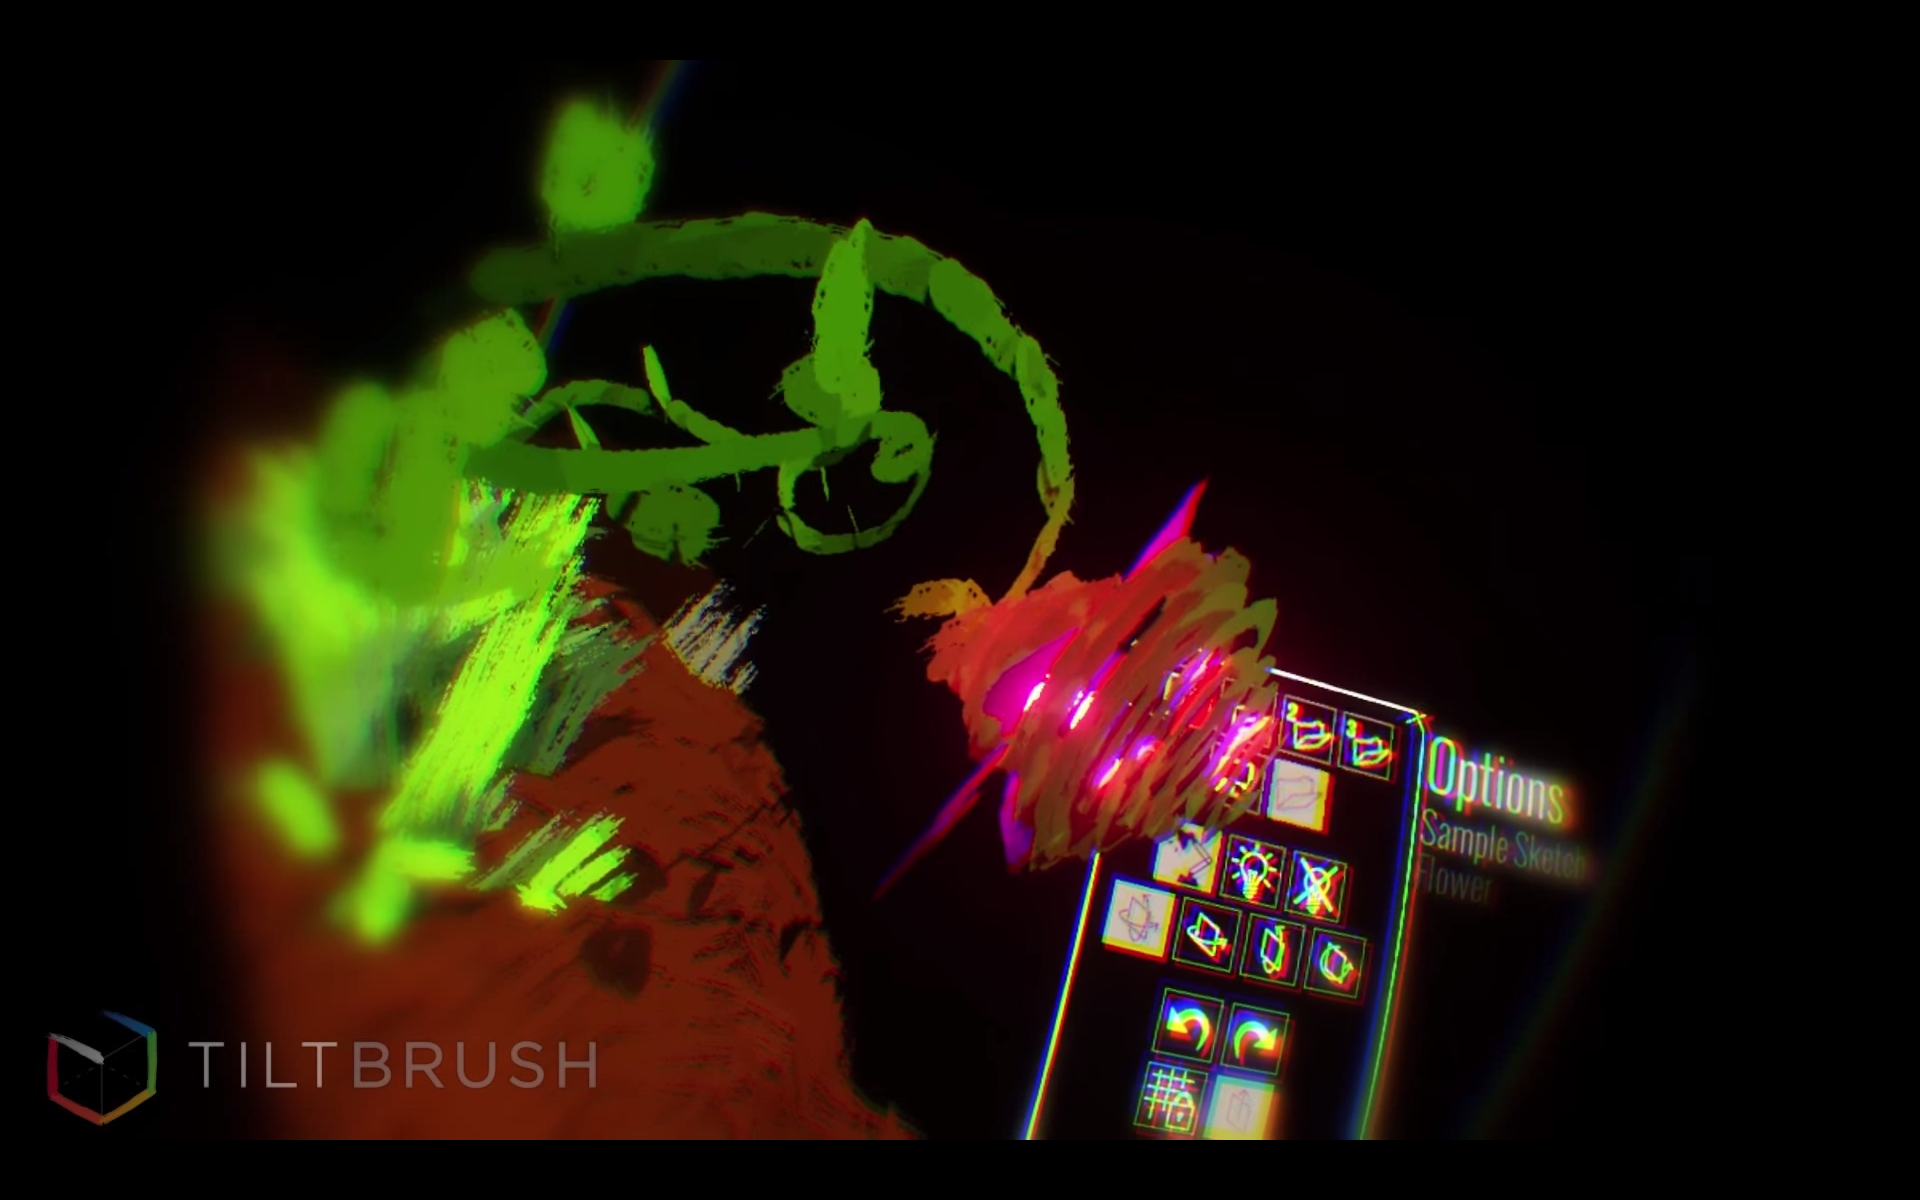
\includegraphics[width=\textwidth]{tiltbrush}
\caption[Virtual Reality Sketching using Tilt Brush]{Virtual reality sketching using Tilt Brush. The user can sketch in a virtual environment in a manner similar to light painting.}
\end{figure}

Recently, there have been two key technologies developed with the intention to immerse the user in a virtual environment or combine virtual images with real environment, termed augmented reality. 
Both of these involve head-mounted displays (HMDs) that display two two-dimensional stereo images.
Despite the images being flat, the system takes advantage of how humans see, such that the user feels the presence of actually being inside of the virtual or augmented reality environments.
The advantage to using these virtual systems is the parallax from the stereo images allows the user to fully be immersed in the space they are working in.
Unfortunately for input tasks, the downside of these systems is that their input methods are essentially drawing in midair; there is no tactile feedback similar to a pen pushing against a piece of paper.
An example of an augmented reality approach to 3-D sketching is Gravity Sketch \autocite{gravitysketch}, and one of a virtual reality approach is Tilt Brush \autocite{tiltbrush}.
Gravity sketch uses a tablet as a sketching surface as well as a tool to manipulate the sketching environment.
Tilt Brush uses a game controller to draw in the air in a manner similar to light painting.

\subsection{3-D Printing}

\begin{figure}
\fbox{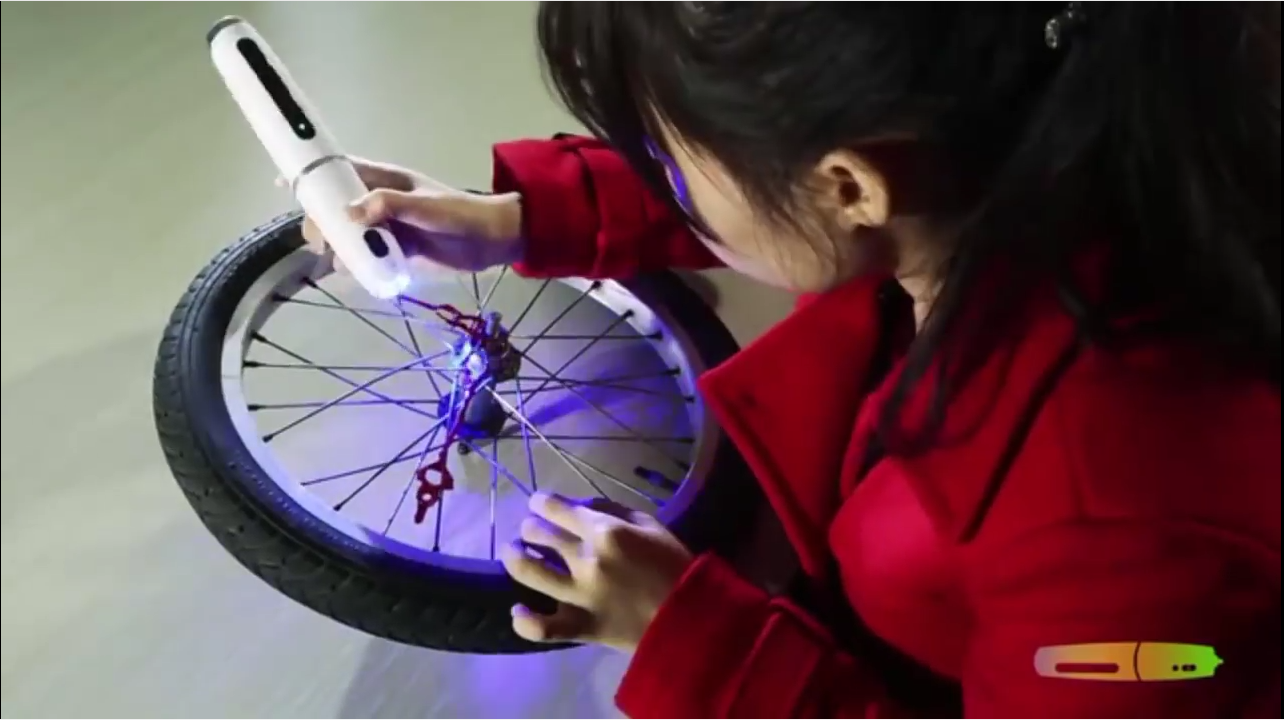
\includegraphics[width=\textwidth]{pq1.png}}
\caption[3D-Drawing using a 3-D Printing Pen]
{3-D drawing using a 3-D printing pen. \autocite{polyes}}
\end{figure}

So far, we have implied 3-D sketching is only possible in virtual environments, due to using the inherent two dimensional techniques artists have developed for centuries.  
However, groups have experimented with using 3-D printing to create pens that can sketch simple 3-D models; examples being the Polyes Q1 Pen \autocite{polyes} and the 3Doodler \autocite{3doodler}.
These pens work similarly to hot glue guns, except instead of glue, the pens secrete ABS plastic that quickly hardens as it exits the tip of the pen.
Like the digital approaches, these pens lack tactile feedback, and rely purely on the user's sight to sketch.
Unfortunately, between the apparent structural instability of even small models created by the pen, as well as the lack of flexibility in the way the pen can be used, it appears that this route is impractical for creating the types of large and intricate structures seen in modern design.